\section{Privacy e dati di locazione}
L'idea alla base è quella di utilizzare la geolocalizzazione per controllare l'accesso. Questo concept presenta diversi vantaggi:
\begin{itemize}
    \item naturale per certi tipi di applicazioni
    \item può permettere di accedere alle risorse ai soli individui di un edificio
\end{itemize}
Migliora sicuramente il controlli dell'accesso con ulteriori capacità di specificare, valutare e rafforzare le condizioni basate sulla locazione.
\begin{center}
    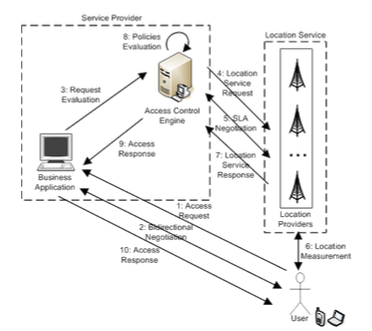
\includegraphics[scale=0.5]{img/lbac.png}
\end{center}
Abbiamo due grandi attori: location provider che gestisce e analizza la posizione, service provider che offre il servizio che può usare la posizione.\\
Tutti i sistemi di geolocalizzazione hanno un margine di errore dovuto a limitazioni tecniche e effetti ambientali. La relevance è una soglia che misura l’accuratezza del dato di location: 0 se non è affidabile, 1 è perfetta e da 0 a 1 se è meno dell'ottimo a causa di errori di misurazione e degradazione artificiale. \\
Mi interessano due valori: 
\begin{itemize}
    \item livello di accuratezza della posizione (\(R_{Eval}\))
    \item livello minimo di accuratezza che il service provider chiede (\(R_{LBAC}\))
\end{itemize}
Le query al Location Service Provider LP possono essere:
\begin{itemize}
    \item \textbf{Range queries}: prendono soltanto dei parametri e restituiscono range, accuratezza, timetout. Esempio: dove si trova Mario Rossi.
    \item \textbf{Boolean queries}: valutano un predicato che ha in input dei parametri e dei valori e restituiscono un booleano, la relavance e un timeout. Esempio: Mario Rossi è in questa posizione?
\end{itemize}
Assumiamo l'esistenza degli elementi seguenti:
\begin{itemize}
    \item utenti: insieme degli identificatori UID che identificano in maniera non ambigua l'utente
    \item aree: insieme di regioni della mappa identificate tramite modelli geometrici o modelli simbolici
\end{itemize}
Esistono principalmente tre classi di condizioni:
\begin{itemize}
    \item position-based: valutano la posizione dell'utente
    \item movement-based: valutano la mobilità dell'utente (velocità, accelerazione, direzione)
    \item interaction-based: relazionano più utenti e/o entità
\end{itemize}
Per quanto riguarda i predicati invece abbiamo:
\begin{itemize}
    \item predicati di posizione:
    \begin{itemize}
        \item inarea(user, area): valuta se l'utente è all'interno di una certa area
        \item disjoint(user, area): valuta se l'utente è fuori dall'area
        \item distance(user, entity, min\_dist, max\_dist): valuta se la distanza tra l'utente e l'entità è tra una distanza minima e una massima
    \end{itemize}
    
    \item predicati di movimento:
    \begin{itemize}
        \item velocity(user, min\_vel, max\_vel): valuta se la velocità dell'utente è tra un valore massimo e un valore minimo
    \end{itemize}
    \item predicati di interazione:
    \begin{itemize}
        \item density(area, min\_num, max\_num): valuta se il numero di utenti presenti nell'area sono all'interno di un numero minimo e un numero massimo
        \item local\_densitu(user, area, min\_num, max\_num): valuta la densità all'interno dell'area dove è presente un determinato utente
    \end{itemize}
\end{itemize}
Ad esempio: inarea(Alice, Milan) = [True, 0.9, 2005-11-09-11:10am] vuol dire che è vero che Alice si trova a Milano con una confidenza del 90\% e che questa informazione è da ritenersi vera fino alle 11:10am del 9 novembre 2005.\\
Le regole del linguaggio basato sulla posizione sono del tipo \(\langle subj\_expr, obj\_expr, action\rangle\) dove:
\begin{itemize}
    \item subj\_expr: formule booleane di termini che specificano condizioni sul soggetto
    \item obj\_expr: formule booleane di termini che specificano condizioni su oggetti
    \item action: azione o classe di azioni alle quali si riferiscono le regole
\end{itemize}
I profili sono referenziati con l'identità dell' utente/oggetto corrispondente. Esistono tuttavia tre variabili predefinite che rendono possibile il riferimento delle condizioni delle regole al richiedente e all'oggetto:
\begin{itemize}
    \item user: identificatore della persona che fa la richiesta
    \item sim: il numero di sim della persona che fa la richiesta
    \item object: identificatore dell'oggetto al quale è richiesto l'accesso
\end{itemize}
\begin{center}
    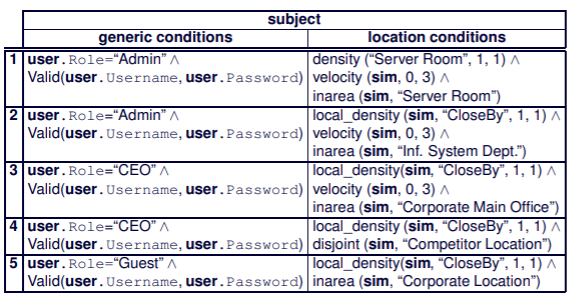
\includegraphics[scale=0.8]{img/locexpress.png}
\end{center}
\subsubsection{Valutazione di LBAC: da \(R_{eval}\) a valori di verità}
I predicati location-based sono formule booleane, mentre la risposta al predicato è nella forma [bool\_value, \(R_{Eval}, timeout\)]. Come facciamo ad ottenere un valore di verità? Possiamo fare uso di tabelle di verità estese che specificano il mapping tra predicati e valori di verità.\\
ACE specifica per ogni predicato e ogni servizio di localizzazione:
\begin{itemize}
    \item rilevanza \(R_{LBAC}\) risultante da due valori soglia (lower, upper) = ((1-\(R_{LBAC}\)), \(R_{LBAC}\))
    \begin{itemize}
        \item \(R_{eval} \leq lower\): !bool\_value è considerato valido
        \item \(R_{eval} \geq lower\): bool\_value è considerato valido
        \item \(lower \leq R_{eval} \leq higher\): la misura è ripetuta
    \end{itemize}
    \item massimo numero di tentativi concessi (MaxTries)
    \begin{center}
        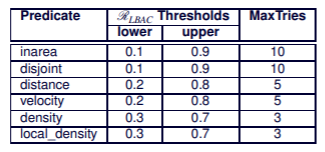
\includegraphics[scale=0.8]{img/lbaceval.png}
    \end{center}
\end{itemize}
LBAC può essere utlrizzato come rinforzo, infatti ricevendo una richiesta di accesso nella forma \(\langle user_id, action, object \rangle\):
\begin{enumerate}
    \item seleziona le regole applicabili
    \item valuta le condizioni generiche
    \item se c'è una regola che è già soddisfatta: garantisci l'accesso
    \item altrimenti valuta le condizioni LB:
    \begin{itemize}
        \item true \(\Longrightarrow\) garantisci l'accesso
        \item false \(\Longrightarrow\) nega l'accesso
        \item unknown \(\Longrightarrow\) nega l'accesso
    \end{itemize}
\end{enumerate}

\subsection{Protezione delle informazioni di locazione}
\begin{center}
    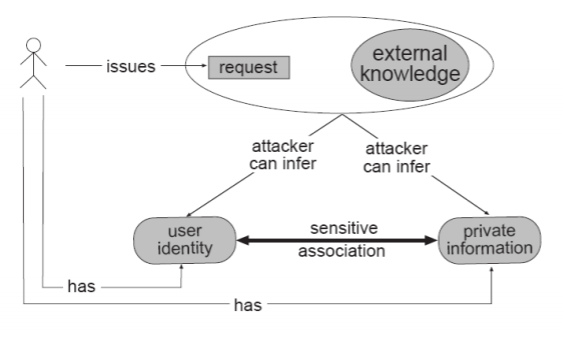
\includegraphics[scale=0.8]{img/locprivacy.png}
\end{center}
Location privacy: il diritto dell'utente di decidere come, quando e per quale scopo le loro informazioni di locazione possono essere rilasciate:
\begin{itemize}
    \item privacy d'identità: protegge l'identità dell'utente associato all'informazione di locazione
    \item privacy di posizione: protegge le informazioni di locazione degli utenti perturbandole
    \item privacy di percorso: protegge il percorso degli utenti
\end{itemize}
Abbiamo a disposizione diversi tipi di soluzioni per proteggere le informazioni sulla posizione:
\begin{itemize}
    \item tecniche anonimity-based: si basano sul concetto di anonimità. Definite in principio per proteggere la privacy di identità, sono meno adatte per proteggere la privacy di posizione, ma più adatte per proteggere la privacy di percorso
    \begin{center}
    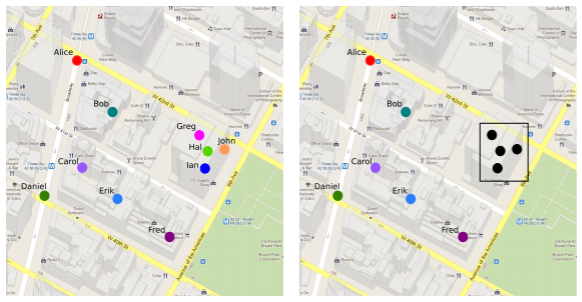
\includegraphics[scale=0.7]{img/anonloc.png}
    \end{center}
    
    \item tecniche obfuscation-based: si basano sul concetto di offuscazione. Definite in principo per proteggere la privacy di posizione, sono meno adatte per proteggere la privacy di identità, ma più adatte per proteggere la privacy di percorso
    \begin{center}
    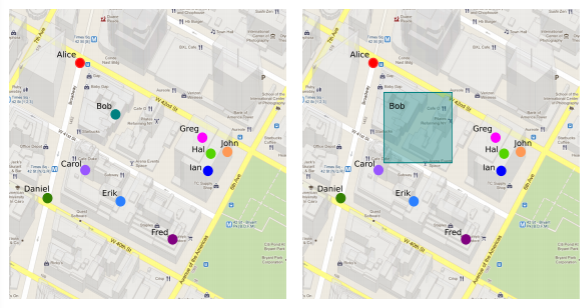
\includegraphics[scale=0.7]{img/obfusloc.png}
    \end{center}
    
    \item tecniche policy-based: si basano sul concetto di privacy policy. Sono ottime per proteggere tutti i tipi di privacy citati sopra
    \begin{center}
    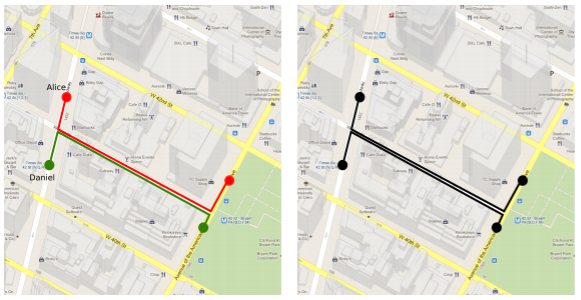
\includegraphics[scale=0.7]{img/pathloc.png}
\end{center}
\end{itemize}
Infrastrutture mobile e basate sui servizi sono caratterizzate da utenti mobile e LBS providers dove:
\begin{itemize}
    \item LBS providers offrono servizi richiedendo il continuo accesso alla posizione degli utenti
    \item utenti mobile rilasciano le loro posizioni ai LBS providers
\end{itemize}
Un LBS provider che analizza le posizioni dell'utente potrebbe effettuare inferenze sulle informazioni sensibili dell'utente e violare la sua privacy.\\
Ci sono tre classi di inferenze possibili:
\begin{enumerate}
    \item sensitive positions (l'utente ha visitato un posto che considera sensibile: user-dependent)
        \begin{center}
    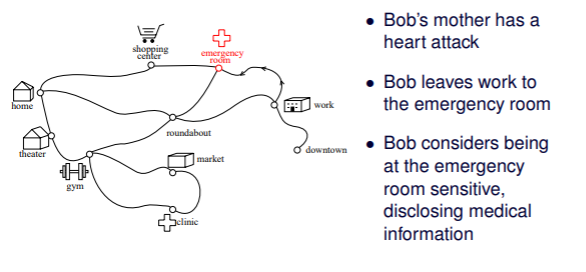
\includegraphics[scale=0.7]{img/senspos.png}
\end{center}
    \item sensitive movements (l'utente ha seguito un percorso che ritiene sensibile: user-dependent)
        \begin{center}
    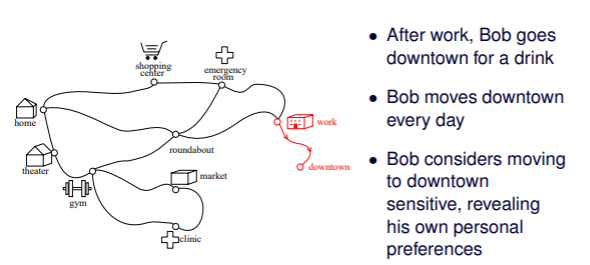
\includegraphics[scale=0.7]{img/sensmov.png}
\end{center}
    \item unusual paths (un utente ha seguito un percorso inusuale per lui: user-independent)
        \begin{center}
    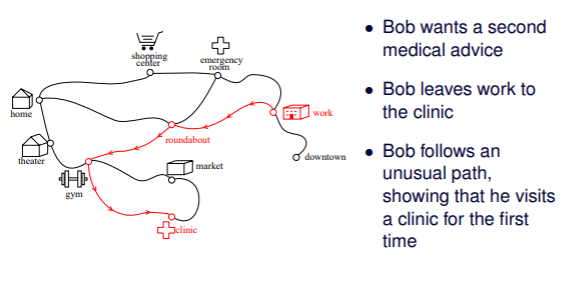
\includegraphics[scale=0.7]{img/unusualpath.png}
\end{center}
\end{enumerate}
La comunicazione tra utenti e providers è mediata da un trusted privacy middleware che:
\begin{enumerate}
    \item valuta le informazioni di locazione degli utenti
    \item calcola il rischio di inferenza
    \item offusca il percorso prima di rilasciarlo se è possibile effettuare delle inferenze (cover stories basato sulle preferenze dell'utente)
\end{enumerate}
La rete viene modellata come un grafo G(V,E) dove V sono le intersezioni tra strade e i punti di interesse ed E sono le strade. \\L'utente, basandosi su questo grafo, può esprimere preferenze di privacy e servizio di qualità.